\documentclass[
	letterpaper, % Paper size, specify a4paper (A4) or letterpaper (US letter)
	10pt, % Default font size, specify 10pt, 11pt or 12pt
]{CSUniSchoolLabReport}

%----------------------------------------------------------------------------------------
%	REPORT INFORMATION
%----------------------------------------------------------------------------------------

\title{Lab One\\ Fundamentals of Electronics \\ EECE2412/3} % Report title

\author{Michael \textsc{Brodskiy}\\ \small \href{mailto:Brodskiy.M@Northeastern.edu}{Brodskiy.M@Northeastern.edu}}

\date{October 1, 2024} % Date of the report

%----------------------------------------------------------------------------------------


\begin{document}

\maketitle % Insert the title, author and date using the information specified above

\begin{center}
	\begin{tabular}{l r}
		Date Performed: & September 17/24, 2024 \\ % Date the experiment was performed
        Partner: & Rahul \textsc{Singh} \\ % Partner names
		Instructor: & Professor \textsc{Onabajo} \\ % Instructor/supervisor
        TAs: & Ming \textsc{Xiang} \& Amr \textsc{Kassab} \\ % Teachers Assistants 
	\end{tabular}
\end{center}

\newpage

\begin{abstract}

  The purpose of this laboratory experiment is to re-orient individuals with the basics of DC power supplies, function generators, and oscilloscopes. This is done through implementation of operational amplifiers (op-amps), which are integrated into various circuits. The limitations of these op-amps are then investigated through integration of an audio amplifier with a microphone.

\end{abstract}

\begin{flushleft}

  \textsc{Keywords:} \underline{power supplies}, \underline{function generators}, \underline{oscilloscopes}, \underline{operational amplifier}, \underline{audio}, \underline{microphone}

\end{flushleft}

\newpage

\tableofcontents

\newpage

\section{Equipment}

Available equipment included:\\

\begin{itemize}

  \item Basic Circuit Components (Capacitors, Resistors, Inductors, etc.)

  \item LM741 Operational Amplifiers

  \item Piezo-electric Speaker

  \item 8-ohm Speaker

  \item Basic Microphone

  \item Keysight EDU36311A Dual DC Power Supply

  \item Keysight EDU33212A Function Generator

  \item Keysight DSOX1204G Digital Oscilloscope

  \item BNC Cables

\end{itemize}

\newpage

\section{Performing the Experiment}

\subsection{Physical Circuitry}\label{physical}

This laboratory experiment begins with the construction of a basic operational amplifier circuit with input from the function generator and readings obtained from the digital oscilloscope at the input and output of the amplifier at channels one and two, respectively. The circuit can be seen in Figure \ref{fig:1} below:

\begin{figure}[H]
  \centering
  \tikzset{every picture/.style={line width=0.75pt}} %set default line width to 0.75pt        

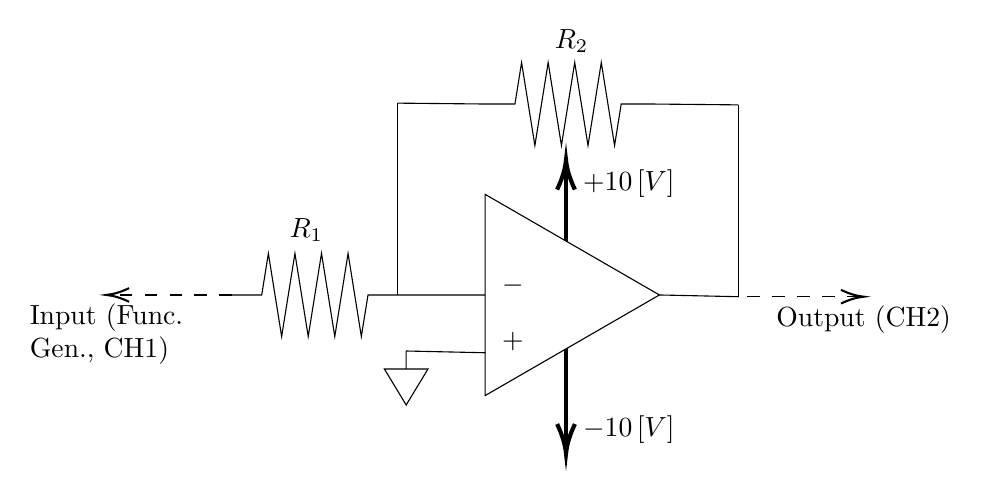
\begin{tikzpicture}[x=0.75pt,y=0.75pt,yscale=-1,xscale=1]
%uncomment if require: \path (0,692); %set diagram left start at 0, and has height of 692

%Straight Lines [id:da973909063029269] 
\draw [line width=1.5]    (290,128.5) -- (290,263.92) ;
\draw [shift={(290,266.92)}, rotate = 270] [color={rgb, 255:red, 0; green, 0; blue, 0 }  ][line width=1.5]    (14.21,-4.28) .. controls (9.04,-1.82) and (4.3,-0.39) .. (0,0) .. controls (4.3,0.39) and (9.04,1.82) .. (14.21,4.28)   ;
\draw [shift={(290,125.5)}, rotate = 90] [color={rgb, 255:red, 0; green, 0; blue, 0 }  ][line width=1.5]    (14.21,-4.28) .. controls (9.04,-1.82) and (4.3,-0.39) .. (0,0) .. controls (4.3,0.39) and (9.04,1.82) .. (14.21,4.28)   ;
%Shape: Ground [id:dp6218025584098273] 
\draw  [fill={rgb, 255:red, 255; green, 255; blue, 255 }  ,fill opacity=1 ] (251,239) -- (335,190.5) -- (251,142) -- (251,239) -- cycle (209,190.5) -- (251,190.5) ;
%Shape: Resistor [id:dp7473730779266806] 
\draw   (129,190.5) -- (143.4,190.5) -- (146.6,170.5) -- (153,210.5) -- (159.4,170.5) -- (165.8,210.5) -- (172.2,170.5) -- (178.6,210.5) -- (185,170.5) -- (191.4,210.5) -- (194.6,190.5) -- (209,190.5) ;
%Straight Lines [id:da4912524923696384] 
\draw    (209,98.08) -- (209,190.5) ;
%Shape: Resistor [id:dp19057956295703093] 
\draw   (251,98.5) -- (265.4,98.5) -- (268.6,78.5) -- (275,118.5) -- (281.4,78.5) -- (287.8,118.5) -- (294.2,78.5) -- (300.6,118.5) -- (307,78.5) -- (313.4,118.5) -- (316.6,98.5) -- (331,98.5) ;
%Straight Lines [id:da44525050708783065] 
\draw    (209,98.08) -- (251,98.5) ;
%Straight Lines [id:da39453577617402236] 
\draw    (331,98.5) -- (373,98.92) ;
%Straight Lines [id:da058156514264413595] 
\draw    (373,98.92) -- (373,191.34) ;
%Straight Lines [id:da29349435917566447] 
\draw    (335,190.5) -- (373,191.34) ;
%Straight Lines [id:da1556742012077138] 
\draw    (213,217.5) -- (251,218.34) ;
%Shape: Ground [id:dp283570639000989] 
\draw   (202.5,226.17) -- (213,243.5) -- (223.5,226.17) -- (202.5,226.17) -- cycle (213,217.5) -- (213,226.17) ;
%Straight Lines [id:da04414817847417474] 
\draw  [dash pattern={on 4.5pt off 4.5pt}]  (129,190.5) -- (70.58,190.5) ;
\draw [shift={(68.58,190.5)}, rotate = 360] [color={rgb, 255:red, 0; green, 0; blue, 0 }  ][line width=0.75]    (10.93,-3.29) .. controls (6.95,-1.4) and (3.31,-0.3) .. (0,0) .. controls (3.31,0.3) and (6.95,1.4) .. (10.93,3.29)   ;
%Straight Lines [id:da6380422554026496] 
\draw  [dash pattern={on 4.5pt off 4.5pt}]  (431.42,191.34) -- (373,191.34) ;
\draw [shift={(433.42,191.34)}, rotate = 180] [color={rgb, 255:red, 0; green, 0; blue, 0 }  ][line width=0.75]    (10.93,-3.29) .. controls (6.95,-1.4) and (3.31,-0.3) .. (0,0) .. controls (3.31,0.3) and (6.95,1.4) .. (10.93,3.29)   ;

% Text Node
\draw (155.6,166.1) node [anchor=south west] [inner sep=0.75pt]    {$R_{1}$};
% Text Node
\draw (283.4,75.1) node [anchor=south west] [inner sep=0.75pt]    {$R_{2}$};
% Text Node
\draw (258,180.4) node [anchor=north west][inner sep=0.75pt]    {$-$};
% Text Node
\draw (258,207.4) node [anchor=north west][inner sep=0.75pt]    {$+$};
% Text Node
\draw (297,128.9) node [anchor=north west][inner sep=0.75pt]    {$+10\left[\text{V}\right]$};
% Text Node
\draw (297,263.52) node [anchor=south west] [inner sep=0.75pt]    {$-10\left[\text{V}\right]$};
% Text Node
\draw (68.58,193.5) node [anchor=north] [inner sep=0.75pt]   [align=left] {Input (Func. \\Gen., CH1)};
% Text Node
\draw (433.42,194.34) node [anchor=north] [inner sep=0.75pt]   [align=left] {Output (CH2)};


\end{tikzpicture}

  \caption{Simple Amplifier Circuit Diagram}
  \label{fig:1}
\end{figure}

Given values of $R_1=10[\si{\kilo\ohm}]$ and $R_2=100[\si{\kilo\ohm}]$, the above circuit was constructed. Furthermore, an input of $.75[\si{V_{pp}}]$ at $8[\si{\kilo\hertz}]$ was specified. The resulting circuit is shown in Figure \ref{fig:2} below (Note the connection of two clips, corresponding to the function generator and oscilloscope channel 1, at the input, and the output to oscilloscope channel 2):

\begin{figure}[H]
  \centering
  \includegraphics[width=.7\textwidth]{Figures/L1F1.jpg}
  \caption{Constructed Circuit Shown in Figure \ref{fig:1}}
  \label{fig:2}
\end{figure}

After passing the given signal through the circuit, the following oscilloscope reading was obtained:

\begin{figure}[H]
  \centering
  \includegraphics[width=.9\textwidth]{Figures/L1F2.jpg}
  \caption{Readings from Circuit Shown in Figure \ref{fig:1}}
  \label{fig:3}
\end{figure}

\begin{figure}[H]
  \centering
  \includegraphics[width=.9\textwidth]{Figures/L1R1.png}
  \caption{Readings from Circuit Shown in Figure \ref{fig:1}}
  \label{fig:4}
\end{figure}

\subsubsection{Determining the Phase Shift Visually}

Looking at Figures \ref{fig:3} and \ref{fig:4}, we may see that the output (green) wave, is a reflection of the input (yellow) wave about the horizontal axis. This corresponds to a phase shift of approximately $180^{\circ}$. This makes sense logically, as the circuit shown in Figure \ref{fig:1} is an inverting amplifier (as the input flows into the negative terminal). This would result in a gain of magnitude 10, but with the opposite sign.

\subsubsection{Determining the Phase Shift Mathematically}

The period may be obtained as:

$$T=\frac{1}{8000}$$
$$T=.125[\si{\milli\second}]$$

The time lag between the two waveforms was measured as $6.08\cdot10^{-5}[\si{\second}]$. We can use this to find the phase shift:

$$\phi=360\left( \frac{6.08\cdot10^{-5}}{.125\cdot10^{-3}} \right)$$
$$\phi=175.1^{\circ}\approx 180^{\circ}$$

The delay is approximately $180^{\circ}$, as expected.

\subsubsection{Maximum Voltage Output}

Using the cursor function on the oscilloscope, the maximum values of the voltage output were obtained as $\pm7.5[\si{\volt}]$ (voltage difference of $15[\si{\volt}]$). Increasing the peak-to-peak voltage results in clipping, as the op-amp voltage supplies are saturated, meaning the output is unable to exceed the supply values.

\begin{figure}[H]
  \centering
  \includegraphics[width=.9\textwidth]{L1R2.png}
  \caption{Saturation of the Op-Amp}
  \label{fig:5}
\end{figure}

\subsubsection{Voltage Swing}

Using the data sheet provided, it was determined that the typical LM741 voltage swing in the given configuration is $\pm14[\si{\volt}]$. Given that the recorded data shows $\pm15[\si{\volt}]$, the voltage swing of the circuit is, more or less, as expected.

\subsubsection{Using a Square Wave}

Integrating a square wave as the input does \underline{not} result in expected output of a square wave. Instead, the output becomes similar to a triangle wave. This is because the amplitude of a square wave switches abruptly, and the internal capacitance of the amplifier is unable to adjust as quickly. Thus, the capacitors take some time to conform to the voltage accordingly.

\begin{figure}[H]
  \centering
  \includegraphics[width=.9\textwidth]{Figures/L1R3.png}
  \caption{Increased Frequency Wave Input}
  \label{fig:6}
\end{figure}

\subsubsection{Increasing the Frequency}

Increasing the frequency with a sinusoidal input results more and more in a triangular wave. This is because operational amplifiers face slew rate limitations, meaning that if the signal oscillates too quickly, it is unable to adjust accordingly (this is similar to why the square wave input approaches a triangular wave, see Figures \ref{fig:6} and \ref{fig:7}).

\begin{figure}[H]
  \centering
  \includegraphics[width=.9\textwidth]{Figures/L1R4.png}
  \caption{Increased Frequency Wave Input}
  \label{fig:7}
\end{figure}

\subsection{Digital Simulation (SPICE)}

The circuit from Section \ref{physical} was reconstructed for digital simulation the schematic is shown in Figure \ref{fig:8} below:

\begin{figure}[H]
  \centering
  \includegraphics[width=.9\textwidth]{Figures/L1Schematic.png}
  \caption{Digital Circuit Schematic}
  \label{fig:8}
\end{figure}

\subsubsection{Verifying Experimental Data}

Running the simulation produced the following output (Figures \ref{fig:9}-\ref{fig:11}):

\begin{figure}[H]
  \centering
  \includegraphics[width=.9\textwidth]{Figures/L1D1.png}
  \caption{Amplitude and Frequency of Input and Output}
  \label{fig:9}
\end{figure}

\begin{figure}[H]
  \centering
  \includegraphics[width=.9\textwidth]{Figures/L1D2.png}
  \caption{Clipping Beginning at About $1.05[\si{\volt}]$ Input (Output Magnitude $>10[\si{\volt}]$)}
  \label{fig:10}
\end{figure}

\begin{figure}[H]
  \centering
  \includegraphics[width=.9\textwidth]{Figures/L1D3.png}
  \caption{Slew Rate Maximum at Approximately $17[\si{\kilo\hertz}]$}
  \label{fig:11}
\end{figure}

It may be observed that the digitally simulated data closely follows the physically acquired data. Specifically, we see that the output has a gain magnitude of 10, with a phase shift of 180$^{\circ}$ (or gain of -10). Furthermore, because of this gain, clipping occurs when the input voltage is greater than $1[\si{\volt}]$. For the simulation, this is visible at $1.05[\si{\volt}]$. The slew rate was observed at $17[\si{\kilo\hertz}]$, which was close to the experimentally obtained value.

\subsubsection{Expected Microphone Circuit Data}

To prepare for the second part of the physical experiment, a digital schematic mimicking the behaviors of the microphone was constructed. The schematic is shown below, along with the expected gain:

\begin{figure}[H]
  \centering
  \includegraphics[width=.9\textwidth]{Figures/L1Schematic2.png}
  \caption{Audio Amplifier Circuit Mock-Up}
  \label{fig:12}
\end{figure}

\begin{figure}[H]
  \centering
  \includegraphics[width=.9\textwidth]{Figures/L1D4.png}
  \caption{Expected Microphone Gain}
  \label{fig:13}
\end{figure}

The gain may be observed as around $-10$, as expected. The final step is to plot the $3[\text{dB}]$ frequency:

\begin{figure}[H]
  \centering
  \includegraphics[width=.9\textwidth]{Figures/L1D5.png}
  \caption{3dB Frequency}
  \label{fig:14}
\end{figure}

From the simulated values, this is the only one that is different from the obtained data. While the physical circuit showed a critical frequency of $3300[\si{\hertz}]$, the simulated data shows $30[\si{\hertz}]$, while calculation produces $22[\si{\hertz}]$.

\subsection{Audio Amplifier Circuit Construction}

The constructed amplifier circuit is shown in Figure \ref{fig:15} below:

\begin{figure}[H]
  \centering
  \includegraphics[width=.9\textwidth]{Figures/L1F3.jpg}
  \caption{Audio Amplifier Circuit}
  \label{fig:15}
\end{figure}

The amplifier produced the following readings:

\begin{figure}[H]
  \centering
  \includegraphics[width=.9\textwidth]{Figures/L1F4.jpg}
  \caption{Audio Amplifier Circuit Readings}
  \label{fig:16}
\end{figure}

Given that the circuit is reading the analog signal from the microphone, there is significant noise produced at the output (green) wave. Furthermore, due to reflections, the gain magnitude was approximately $5$, instead of the expected $10$.

\subsubsection{Using an 8-ohm Speaker}

The implementation of an 8-ohm Speaker resulted in a louder output from the microphone. This is expected, as the speaker has a lower impedance than the piezo-electric speaker, but receives the same current flow. Thus, the perceived volume is louder.

\newpage

\section{Conclusion}

Throughout the laboratory experiment, a test circuit was constructed as a refresher on power supplies, waveform generators, oscilloscopes, and operational amplifiers. These concepts were then confirmed virtually through SPICE circuit construction and simulation. Finally, the concepts were synthesized in the construction of a final audio amplifier circuit.

\end{document}
